%%%%%%%%%%%%%%%%%% HEAT EQUATION 1D %%%%%%%%%%%%%%%%%%

\newcommand{\HeatEquationOneD}[1]
{
	\onegraph{$x$}{$u(x,t)$}{ xmax = 1, xmin = -1}
	%
	{./doc/chapters/Initial_Boundary_Value_Problem/figures/Heat_Equation_1D/Heat_Equation_1D.dat}{$t=0$,$t=1$,$t=2$,$t=4$}
	{1,2,3,4}{ #1 }
}





\newcommand{\HeatEquationOneDFlux}[1]
{
	\onegraph{$x$}{$\pdv*{u}{x}$}{ xmax = 1, xmin = -1}
	%
	{./doc/chapters/Initial_Boundary_Value_Problem/figures/Heat_Equation_1D/Heat_Equation_1D_Flux.dat}{$t=0$,$t=1$,$t=2$,$t=4$}
	{1,2,3,4}{ #1 }
}


%%%%%%%%%%%%%%%%%% ADVECTION DIFFUSION EQUATION 1D %%%%%%%%%%%%%%%%%%

\newcommand{\AdvectionEquationOneD}[1]
{
	\onegraph{$x$}{$u(x,t)$}{ mark repeat = 5, xmax = 1, xmin = -1, ymin = 0, legend pos = north west}
	%
	{./doc/chapters/Initial_Boundary_Value_Problem/figures/Advection_diffusion_1D/Advection_diffusion_1D.dat}{$t=0.0$,$t=0.5$,$t=1.0$,$t=2.0$}
	{1,2,3,4}{ #1 }
}

\newcommand{\AdvectionEquationOneDFlux}[1]
{
	\onegraph{$x$}{$u(x,t)$}{ mark repeat = 5, xmax = 1, xmin = -1, ymin = -10, legend pos = south west}
	%
	{./doc/chapters/Initial_Boundary_Value_Problem/figures/Advection_diffusion_1D/Advection_diffusion_1D_Flux.dat}{$t=0.0$,$t=0.5$,$t=1.0$,$t=2.0$}
	{1,2,3,4}{ #1 }
}

%%%%%%%%%%%%%%%%%% HEAT EQUATION 2D %%%%%%%%%%%%%%%%%%

\newcommand{\HeatEqTwoDzero}[1]
{   
	\onecontour{ xlabel = $x$, ylabel = $y$, colormap/blackwhite}{11}
	%
	{./doc/chapters/Initial_Boundary_Value_Problem/figures/Heat_equation_2D/U0.dat}
	{contour filled={number = 25}}
	{ #1 }
}

\newcommand{\HeatEqTwoDone}[1]
{   
	\onecontour{ xlabel = $x$, ylabel = $y$, colormap/blackwhite, point meta max=1}{11}
	%
	{./doc/chapters/Initial_Boundary_Value_Problem/figures/Heat_equation_2D/U1.dat}
	{contour filled={number = 25}}
	{ #1 }
}

\newcommand{\HeatEqTwoDTwo}[1]
{   
	\onecontour{ xlabel = $x$, ylabel = $y$, colormap/blackwhite, point meta max=1}{11}
	%
	{./doc/chapters/Initial_Boundary_Value_Problem/figures/Heat_equation_2D/U2.dat}
	{contour filled={number = 25}}{ #1 }
}

\newcommand{\HeatEqTwoDThree}[1]
{   
	\onecontour{ xlabel = $x$, ylabel = $y$, colormap/blackwhite, point meta max=1}{11}
	%
	{./doc/chapters/Initial_Boundary_Value_Problem/figures/Heat_equation_2D/U3.dat}
	{contour filled={number = 25}}{ #1 }
}


%%%%%%%%%%%%%%%%%% ADVECTION DIFFUSION EQUATION 2D %%%%%%%%%%%%%%%%%%

\newcommand{\AdvectionEqTwoDzero}[1]
{   
	\onecontour{ xlabel = $x$, ylabel = $y$, colormap/blackwhite}{21}
	%
	{./doc/chapters/Initial_Boundary_Value_Problem/figures/Advection_diffusion_2D/U0.dat}
	{contour filled={number = 25}}{ #1 }
}

\newcommand{\AdvectionEqTwoDone}[1]
{   
	\onecontour{ xlabel = $x$, ylabel = $y$, colormap/blackwhite, point meta max=1}{21}
	%
	{./doc/chapters/Initial_Boundary_Value_Problem/figures/Advection_diffusion_2D/U1.dat}
	{contour filled={number = 25}}{ #1 }
}

\newcommand{\AdvectionEqTwoDTwo}[1]
{   
	\onecontour{ xlabel = $x$, ylabel = $y$, colormap/blackwhite, point meta max=1}{21}
	%
	{./doc/chapters/Initial_Boundary_Value_Problem/figures/Advection_diffusion_2D/U2.dat}
	{contour filled={number = 25}}{ #1 }
}

\newcommand{\AdvectionEqTwoDThree}[1]
{   
	\onecontour{ xlabel = $x$, ylabel = $y$, colormap/blackwhite, point meta max=1}{21}
	%
	{./doc/chapters/Initial_Boundary_Value_Problem/figures/Advection_diffusion_2D/U3.dat}
	{contour filled={number = 25}}{ #1 }
}


%%%%%%%%%%%%%%%%%% WAVES EQUATION 1D %%%%%%%%%%%%%%%%%%

\newcommand{\WavesEquationOneD}[1]
{
	\onegraph{$x$}{$u(x,t)$}{ mark repeat = 5, xmax = 1, xmin = -1, ymin = -1.65, legend pos = south west, legend columns = 2}
	%
	{./doc/chapters/Initial_Boundary_Value_Problem/figures/Waves_Equation_1D/Waves_Equation_1D.dat}{$t=0.0$,$t=1.1$,$t=2.5$,$t=4.5$}
	{1,2,3,4}{ #1 }
}





\newcommand{\WavesEquationOneDAcceleration}[1]
{
	\onegraph{$x$}{$\pdv*[2]{u}{x}$}{ mark repeat = 5, xmax = 1, xmin = -1, ymin = -50, legend pos = south west, legend columns = 2 }
	%
    {./doc/chapters/Initial_Boundary_Value_Problem/figures/Waves_Equation_1D/Waves_Equation_1D_acceleration.dat}{$t=0.0$,$t=1.1$,$t=2.5$,$t=4.5$}
    {1,2,3,4}{ #1 }
}


%%%%%%%%%%%%%%%%%% WAVES EQUATION 2D %%%%%%%%%%%%%%%%%%

\newcommand{\WavesEqTwoDzero}[1]
{   
	\onecontour{ xlabel = $x$, ylabel = $y$, colormap/blackwhite, point meta max=1, point meta min=-0.53}{21}
	%
	{./doc/chapters/Initial_Boundary_Value_Problem/figures/Waves_equation_2D/U0.dat}
	{contour filled={number = 25}}{ #1 }
}

\newcommand{\WavesEqTwoDone}[1]
{   
	\onecontour{ xlabel = $x$, ylabel = $y$, colormap/blackwhite, point meta max=1, point meta min=-0.53}{21}
	%
	{./doc/chapters/Initial_Boundary_Value_Problem/figures/Waves_equation_2D/U1.dat}
	{contour filled={number = 25}}{ #1 }
}

\newcommand{\WavesEqTwoDTwo}[1]
{   
	\onecontour{ xlabel = $x$, ylabel = $y$, colormap/blackwhite, point meta max=1, point meta min=-0.53}{21}
	%
	{./doc/chapters/Initial_Boundary_Value_Problem/figures/Waves_equation_2D/U2.dat}
	{contour filled={number = 25}}{ #1 }
}

\newcommand{\WavesEqTwoDThree}[1]
{   
	\onecontour{ xlabel = $x$, ylabel = $y$, colormap/blackwhite, point meta max=1, point meta min=-0.53}{21}
	%
	{./doc/chapters/Initial_Boundary_Value_Problem/figures/Waves_equation_2D/U3.dat}
	{contour filled={number = 25}}{ #1 }
}


%%%%%%%%%%%%%%%%%% PLATE VIBRATION (PULSE) %%%%%%%%%%%%%%%%%%

\newcommand{\PlateVibrationzero}[1]
{   
	\onecontour{ xlabel = $x$, ylabel = $y$, colormap/blackwhite, point meta max=0.05, point meta min=-0.044}{21}
	%
	{./doc/chapters/Initial_Boundary_Value_Problem/figures/Linear_Vibrations_Plates_Pulse/U0.dat}
	{contour filled={number = 15}}{ #1 }
}

\newcommand{\PlateVibrationOne}[1]
{   
	\onecontour{ xlabel = $x$, ylabel = $y$, colormap/blackwhite,  point meta max=0.05, point meta min=-0.044}{21}
	%
	{./doc/chapters/Initial_Boundary_Value_Problem/figures/Linear_Vibrations_Plates_Pulse/U1.dat}
	{contour filled={number = 15}}{ #1 }
}

\newcommand{\PlateVibrationTwo}[1]
{   
	\onecontour{ xlabel = $x$, ylabel = $y$, colormap/blackwhite,  point meta max=0.05, point meta min=-0.044}{21}
	%
	{./doc/chapters/Initial_Boundary_Value_Problem/figures/Linear_Vibrations_Plates_Pulse/U2.dat}
	{contour filled={number = 15}}{ #1 }
}

\newcommand{\PlateVibrationThree}[1]
{   
	\onecontour{ xlabel = $x$, ylabel = $y$, colormap/blackwhite, point meta max=0.05, point meta min=-0.044}{21}
	%
	{./doc/chapters/Initial_Boundary_Value_Problem/figures/Linear_Vibrations_Plates_Pulse/U3.dat}
	{contour filled={number = 15}}{ #1 }
}

\newcommand{\PlateVibrationFour}[1]
{   
	\onecontour{ xlabel = $x$, ylabel = $y$, colormap/blackwhite, point meta max=0.05, point meta min=-0.044}{21}
	%
	{./doc/chapters/Initial_Boundary_Value_Problem/figures/Linear_Vibrations_Plates_Pulse/U4.dat}
	{contour filled={number = 15}}{ #1 }
}


%%%%%%%%%%%% DEVELOPER FIGURES %%%%%%%%%%%%%%%%%%%%%%%%%%%%%

\newcommand{\IBVPmethodlines}
{
	\begin{figure}[htpb]
		\centering
		\begin{tikzpicture}
		\tikzstyle{every node}=[align=center]
		\node(d) at ( 1.5,-7.5 ) {Temporal \\ discretization};
		\node(e) at ( 1.5, -2.5 ) {Spatial \\ discretization};
		
		\tikzstyle{every node}=[draw, align=center, rectangle ]
		
		\node(a) at (0,0) {\textbf{IBVP} \\ \\$ \dfrac{\partial \vect{u}}{\partial t} = \vect{\mathcal{L}}(\vect{x},t,\vect{u}),$ \\ $ $ \\ $\vect{u}(\vect{x},0)=\vect{u}_0(\vect{x}), $ \\ + \\ $\eval{\vect{h}(\vect{x},t,\vect{u})}_{\partial \Omega} = 0.$};
		
		\node(b) at (0,-5) {\textbf{Cauchy Problem} \\ \\$ \dfrac{\dd U_{\Omega}}{\dd t} = F(U;t),$ \\ $ $ \\ $U(0)=U^0, $\\ + \\ $\eval{H(U;t)}_{\partial \Omega} = 0.$ };
		
		\node(c) at (0,-10) {\textbf{Temporal scheme} \\ \\$G({U}_{\Omega}^{n+1}, {U}^{n}, \ldots {U}^{n+1-s};t_n, \Delta t)={F}({U}^n;t_n) ,$\\ + \\ $\eval{H(U^n;t)}_{\partial \Omega} = 0.$ 
			\\ \\ where $U^0$ is known.};
		
		\foreach \from/\to in {a/b, b/c}
		\draw [->, thick = 1 pt] (\from) -- (\to) ;
		
		\end{tikzpicture}
		\caption{Line method for initial value boundary problems.} 
		\label{fig:IBVPmethodlines}
	\end{figure}
}


\newcommand{\IBVPalgorithm}
{
 \begin{figure}[H]
 	\hspace{-0.5cm}
 	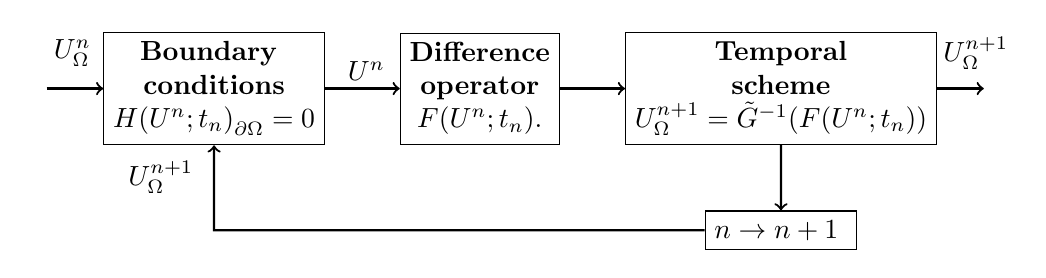
\begin{tikzpicture}[scale=0.9]
 	\node[rectangle](0) at (-2.5,0) {};
 	\node[rectangle](un) at (-2.,0.5) {$U_{\Omega}^{n}$};
 	\node[rectangle](f) at (11,0) {};
 	\node[rectangle](un1) at (10.75,0.5) {$U_{\Omega}^{n+1}$};
 	\node[rectangle](e) at (-0.75,-1.25) {$U_{\Omega}^{n+1}$};
 	\node(ab) at (2.15,0.25) {${U^n}$};
 	
 	\tikzstyle{every node}=[draw, align=center, rectangle ]
 	\node(a) at (0,0) {\textbf{Boundary } \\ \textbf{conditions} \\ 
 		$\eval{H(U^n;t_n)}_{\partial \Omega} = 0 $};
 	
 	\node(b) at (3.75,0) {\textbf{Difference} \\ \textbf{operator} \\ $ F(U^n; t_n)$.};
 	
 	\node(c) at (8,0) {\textbf{Temporal} \\ \textbf{scheme} \\ $U_{\Omega}^{n+1} = \tilde{G}^{-1}(F(U^n; t_n))$ 
 	};
 	
 	\node(d) at (8,-2) {$n \rightarrow n +1 $ 
 	};
 	
 	\draw [->, thick = 1 pt] (d) -- (0,-2) -- (a) ;
 	
 	\foreach \from/\to in {0/a,a/b,b/c,c/d,c/f}
 	\draw [->, thick = 1 pt] (\from) -- (\to) ;%node[midway] {\from--\to};
 	
 	
 	\end{tikzpicture}
 	\caption{Resolution algorithm for initial value boundary problems.}
 	\label{fig:IBVPalgorithm}
 \end{figure}
}


\newcommand{\IVBPerrors}
{
	\begin{figure}[htpb]
		\centering
		\begin{tikzpicture}
		%\tikzstyle{every node}=[align=center]
		%\node(d) at (  7,-2.5 ) {Temporal \\ discretization};
		%\node(e) at ( 2.5, 0.5 ) {Spatial \\ discretization};
		
		\tikzstyle{every node}=[draw, align=center, rectangle ]
		
		\node(a) at (0,0) {\textbf{IVBP} \\ \\$ \dfrac{\partial \vect{u}}{\partial t} = \vect{\mathcal{L}}(\vect{x},t,\vect{u}),$ \\ $ $ \\ $\vect{u}(\vect{x},0)=\vect{u}_0(\vect{x}), $ \\ + \\ $\eval{\vect{h}(\vect{x},t,\vect{u})}_{\partial \Omega} = 0.$};
		
		\node(b) at (0,-5) {\textbf{Cauchy Problem} \\ \\$ \dfrac{\dd U_{\Omega}}{\dd t} = AU + b,$ \\ $ $ \\ $U(0)=U^0, $\\ + \\ $\eval{H(U;t)}_{\partial \Omega} = 0.$ };
		
		\node(c) at (0,-10) {\textbf{Temporal scheme} \\ \\${U}_{\Omega}^{n+1}= {U}_{\Omega}^{n}+ \Delta t (AU ^n + b^n) ,$\\ + \\ $\eval{H(U^n;t)}_{\partial \Omega} = 0.$ 
			\\ \\ where $U^0$ is known.};
		
		\node(ab) at (5,-2.5)  {\textbf{Spatial error}\\ \\$\dfrac{\dd E}{\dd t} = A E + R$};
		
		\node(bc) at (5,-7.5)  {\textbf{Temporal error}\\ \\$E^{n+1} = B E^{n} + T^{n}$};
		
		\node(ce) at (5,-12)  {\textbf{Total error}\\ \\$E_T = E + E^{n}$};
		
		
		
		\foreach \from/\to in {a/b, b/c, a/ab, ab/b, b/bc, bc/c, c/ce}
		\draw [->, thick = 1 pt] (\from) -- (\to) ;%node[midway] {\from--\to};
		
		%\draw [->, thick = 1 pt] (b) -- (5.5,-2.5) -- (0,-2.5) -- (0,-5) -- (c);
		\end{tikzpicture}
		\caption{Errors during the numerical resolution of initial value boundary problems.}
		\label{fig:IBVPerrors}
	\end{figure}

}